\documentclass[conference]{IEEEtran}
\usepackage[utf8]{inputenc}
\usepackage[brazil]{babel}
\usepackage{graphicx}
\usepackage{booktabs}
\usepackage{amsmath}
\usepackage{cite}
\usepackage{url}

% Atualize após rodar stats_test.py e plots.py
\newcommand{\mediaFZero}{0,000}
\newcommand{\mediaFOne}{0,000}
\newcommand{\pvalor}{0,000}
\newcommand{\cohend}{0,00}
\newcommand{\conclusaoStats}{%
  [Cole aqui a conclusão de \texttt{results/stats.txt}]
}

\begin{document}

\title{Estudo Comparativo de Ensemble Learning versus Modelo Único na Classificação de Pneumonia em Radiografias de Tórax}

\author{\IEEEauthorblockN{Seu Nome}
\IEEEauthorblockA{Curso de Ciência da Computação\\
Disciplina: Inteligência Artificial (Eletiva)\\
Instituição -- E-mail: seu.email@instituicao.edu.br}
}

\maketitle

\begin{abstract}
Este trabalho compara duas abordagens de deep learning para classificação binária de pneumonia em radiografias de tórax (dataset PneumoniaMNIST): (i) cenário de hipótese nula (H0), com um único classificador ResNet18 fine-tuned a partir de pesos ImageNet; e (ii) cenário de hipótese alternativa (H1), combinando transfer learning com ensemble por votação suave entre ResNet18, MobileNetV2 e EfficientNet-B0. Foram realizadas 30 simulações pareadas variando a semente aleatória. A métrica principal é o F1-score, adequada ao desbalanceamento das classes. Testes estatísticos pareados (Shapiro-Wilk, $t$ pareado ou Wilcoxon) avaliam se H1 supera H0 com $\alpha=0{,}05$. Os resultados indicam \conclusaoStats
\end{abstract}

\begin{IEEEkeywords}
Visão computacional, transfer learning, ensemble learning, PneumoniaMNIST, teste de hipótese.
\end{IEEEkeywords}

\section{Introdução}
A detecção automática de pneumonia em radiografias de tórax é relevante para triagem clínica e apoio à decisão. Redes neurais convolucionais (CNNs) alcançam desempenho competitivo quando combinadas com transfer learning a partir de bases naturais de imagens~\cite{he2016deep,pan2010survey}. Ensemble learning agrega predições de múltiplos modelos, frequentemente reduzindo variância~\cite{dietterich2000ensemble}, ao custo de maior tempo de treino e inferência.

A disciplina eletiva de Inteligência Artificial exige um estudo comparativo entre três técnicas vistas em sala, em dois cenários que diferem na terceira técnica. Fixamos classificação de imagens (técnica A) e transfer learning (técnica B). No cenário H0, a técnica C é um modelo único; no cenário H1, a técnica C alternativa é ensemble learning. Objetivamos inferir estatisticamente qual abordagem é mais eficaz.

\section{Fundamentação Teórica}

\subsection{Classificação em visão computacional}
Trata-se de mapear imagens $x$ para rótulos discretos $y$. Utilizamos CNNs com camada final softmax sobre duas classes (normal vs.\ pneumonia).

\subsection{Transfer learning}
Inicializamos pesos pré-treinados na ImageNet e realizamos fine-tuning no domínio médico, acelerando convergência e melhorando generalização com poucos dados~\cite{pan2010survey}.

\subsection{Ensemble learning}
No cenário H1, cada modelo produz probabilidades $p_i(y{=}1 \mid x)$; a votação suave define $p_{\mathrm{ens}} = \frac{1}{M}\sum_{i=1}^{M} p_i$. A classe predita usa limiar 0,5.

\section{Metodologia}

\subsection{Dataset e pré-processamento}
Utilizamos PneumoniaMNIST~\cite{yang2023medmnist}, subset MedMNIST com imagens $64\times64$. Réplicas em três canais e normalização ImageNet. Divisões oficiais de treino, validação e teste são mantidas.

\subsection{Modelos}
H0: ResNet18~\cite{he2016deep}. H1: ensemble de ResNet18, MobileNetV2~\cite{sandler2018mobilenetv2} e EfficientNet-B0~\cite{tan2019efficientnet}, todos com cabeça binária.

\subsection{Treinamento}
Otimizador Adam ($\mathrm{lr}=10^{-3}$), batch 128, até 5 épocas com early stopping (paciência 3) pela loss de validação. Em cada simulação $s \in \{0,\ldots,29\}$, a mesma ResNet18 é treinada uma vez e reutilizada em H0 e H1 (pareamento).

\subsection{Métricas e hipóteses}
Métricas: acurácia, F1 (principal) e AUC-ROC. Hipóteses unilaterais sobre F1: $H_0: \mu_{\mathrm{H1}} \leq \mu_{\mathrm{H0}}$ vs.\ $H_1: \mu_{\mathrm{H1}} > \mu_{\mathrm{H0}}$, $\alpha=0{,}05$. Normalidade das diferenças verificada por Shapiro-Wilk; em caso positivo, $t$ pareado; caso contrário, Wilcoxon. Reportamos Cohen's $d$~\cite{cohen1988statistical} e IC 95\% da diferença média.

\section{Resultados}

\begin{table}[t]
\centering
\caption{Resumo das métricas (média $\pm$ desvio padrão, 30 simulações). Atualize com \texttt{results/results.csv}.}
\label{tab:metricas}
\begin{tabular}{lccc}
\toprule
Cenário & Acurácia & F1 & AUC \\
\midrule
H0 (modelo único) & -- & \mediaFZero & -- \\
H1 (ensemble)     & -- & \mediaFOne  & -- \\
\bottomrule
\end{tabular}
\end{table}

\begin{figure}[t]
\centering
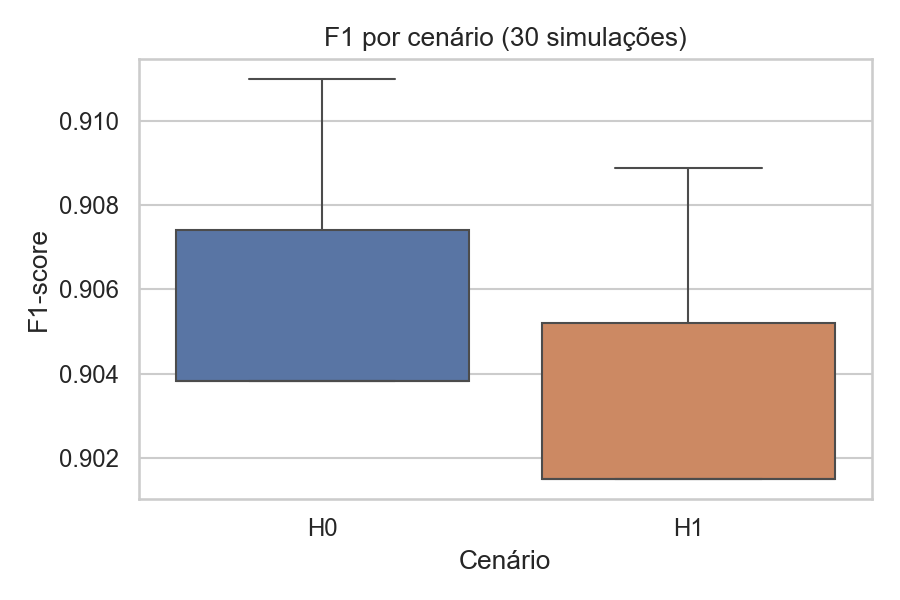
\includegraphics[width=\linewidth]{../results/figs/f1_boxplot.png}
\caption{Distribuição do F1-score por cenário.}
\label{fig:box}
\end{figure}

\begin{figure}[t]
\centering
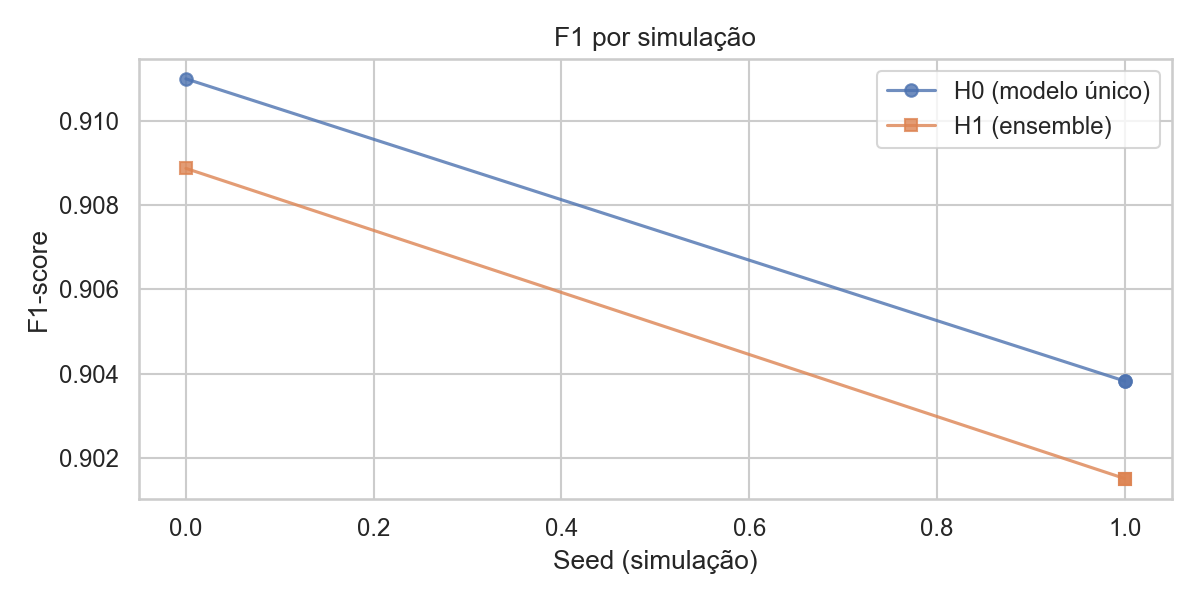
\includegraphics[width=\linewidth]{../results/figs/f1_por_seed.png}
\caption{F1 por simulação (seed), evidenciando pareamento.}
\label{fig:lines}
\end{figure}

\begin{figure}[t]
\centering
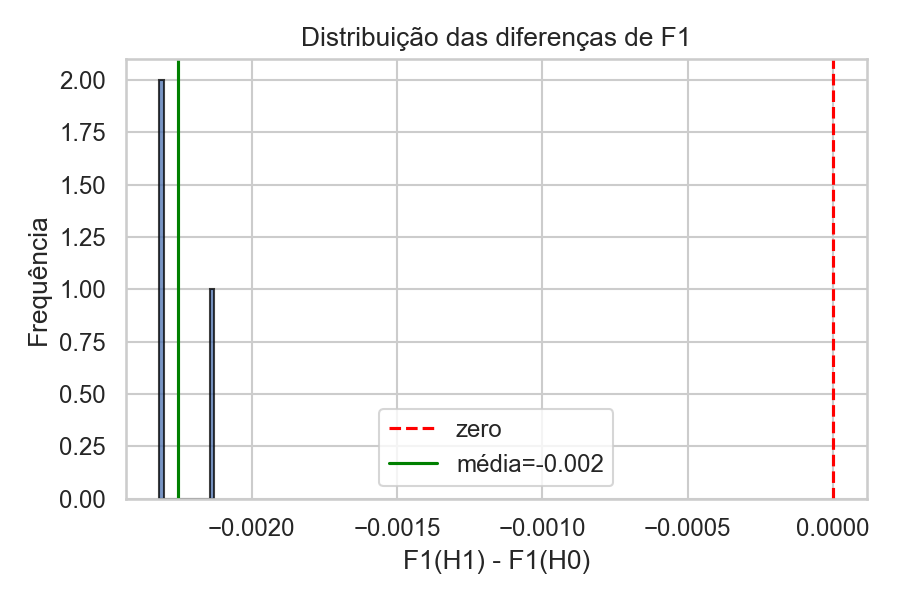
\includegraphics[width=\linewidth]{../results/figs/f1_diff_hist.png}
\caption{Histograma das diferenças F1(H1)$-$F1(H0).}
\label{fig:hist}
\end{figure}

\begin{figure}[t]
\centering
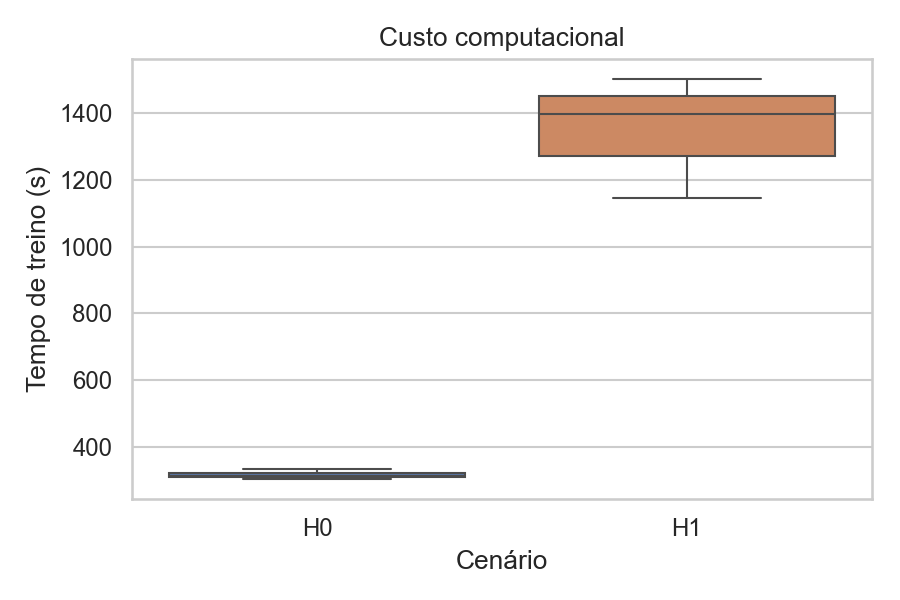
\includegraphics[width=\linewidth]{../results/figs/tempo_treino.png}
\caption{Tempo de treino por cenário.}
\label{fig:time}
\end{figure}

O teste estatístico resultou em $p=\pvalor$ (unilateral), com Cohen's $d=\cohend$. \conclusaoStats

\section{Discussão}
O ensemble tende a combinar representações complementares (ResNet, MobileNet, EfficientNet), porém exige treinar três arquiteturas (Fig.~\ref{fig:time}). Em simulações onde H1 não supera H0 de forma significativa, o ganho marginal pode não justificar o custo em ambientes com restrição de tempo ou energia. Limitações incluem imagens de baixa resolução e ausência de calibração de limiar por validação.

\section{Conclusão}
Comparamos modelo único versus ensemble sob transfer learning na PneumoniaMNIST, com 30 simulações pareadas e inferência estatística formal. O código reprodutível está disponível no repositório do projeto. A decisão entre H0 e H1 deve considerar tanto significância estatística do F1 quanto custo computacional.

\bibliographystyle{IEEEtran}
\bibliography{refs}

\end{document}
